%%%%%%%%%%%%%%%%%%%%%%%%%%%%%%%%%%%%%%%%%%%%%%%%%%%%%%%%%%%%%%%%%
% Contents : The reconciliation chapter
% Translation of the French & English versions and extracts from the German version 2.0.0 - thanks to Martin Stromberger
% $Id : 10-grisbi-manuel-de.tex, v 3.0 2026/08 Dominique Brochard
%%%%%%%%%%%%%%%%%%%%%%%%%%%%%%%%%%%%%%%%%%%%%%%%%%%%%%%%%%%%%%%%%


\chapter{Planer\label{plannedtransactions}}
%\chapter{Scheduler\label{plannedtransactions}}
%\chapter{Échéancier\label{plannedtransactions}}

Mit dem Planer können Sie wiederkehrende Buchungen mit bestimmten Daten oder Zeitintervallen planen. Sobald eine Buchung in den Planer eingegeben wurde, kopiert Grisbi die geplante Buchung automatisch in die Buchungsliste, sobald ihr \indexword{Fälligkeitsdatum}\index{Fälligkeitsdatum} erreicht ist.
%The scheduler allows you to plan recurring transactions with specific dates or time intervals. Once a transaction is entered into the scheduler, Grisbi automatically copies the scheduled transaction to the transaction list as soon as its \indexword{due date}\index{due!date} is reached.
%L'échéancier permet de planifier des opérations qui reviennent régulièrement avec des dates ou des intervalles de temps déterminés. Une fois qu'une opération est enregistrée dans l'échéancier, Grisbi recopie automatiquement l'opération planifiée dans la liste des opérations dès que sa \indexword{date d'échéance}\index{date!échéance} est atteinte.


Darüber hinaus zeigt Grisbi auf der Startseite Benachrichtigungen an, wenn die Fälligkeitstermine für diese Buchungen anstehen (siehe Abschnitt \vref{home-details-homepage}, \menus{Startseite}).
%Furthermore, Grisbi displays alerts on the home page when the due dates for these transactions are due (see the section \vref{home-details-homepage}, \menus{Homepage}).
%De plus, Grisbi affiche dans la page d'accueil des alertes au déclenchement des échéances de ces opérations (voir la section \vref{home-details-homepage}, \menus{Affichage de la page d'accueil}).

% espace pour changement de thème

\vspacepdf{2mm}
Um auf geplante Buchungen zuzugreifen, klicken Sie im Navigationsbereich auf \menus{Planer} oder wählen Sie in der Informationsleiste \menus{Geplante Buchungen} aus (siehe Abschnitt \vref{home}, \menus{Startseite}).
%To access scheduled transactions, click on \menus{Scheduler} in the navigation panel, or select \menus{Scheduled transactions} from the information bar (see the chapter \vref{home}, \menus{Home}).
%Pour accéder aux opérations planifiées, cliquez sur \menus{Échéancier} dans le panneau de navigation, ou sélectionnez \menus{Opérations planifiées} avec la barre d'information (voir le chapitre \vref{home}, \menus{Accueil}).

\begin{figure}[htbp]
	\begin{center}
		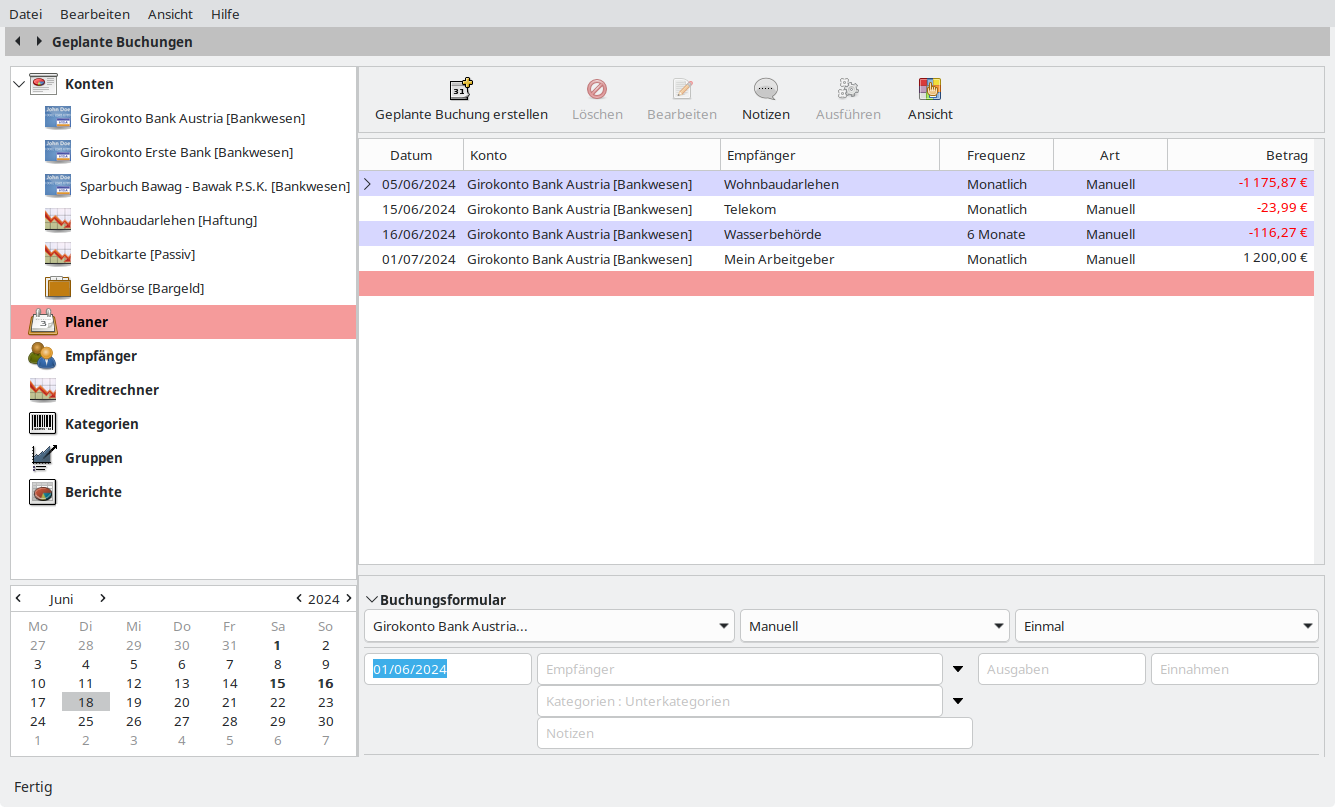
\includegraphics[width=0.95\textwidth]{image/screenshot/planned_transactions_display}
	\end{center}
	\caption{Geplante Transaktionen anzeigen}
	%\caption{Viewing scheduled transactions}
	%\caption{Affichage des opérations planifiées}
	\label{planned-transactions-display-img}
\end{figure}

Am unteren Rand des Navigationsbereichs wird ein Kalender angezeigt, und der Detailbereich enthält nun drei Elemente\refimage{planned-transactions-display-img}:
%A calendar appears at the bottom of the navigation panel, and the details panel then contains three elements\refimage{planned-transactions-display-img}:
%Un calendrier s'affiche en bas du panneau de navigation, et le pavé des détails possède alors trois éléments\refimage{planned-transactions-display-img}:
\begin{itemize}
	\item die Werkzeugliste;
	%\item the toolbar;
	%\item la barre d'outils;
	\item die Liste der geplanten Buchungen;
	%\item the list of scheduled transactions;
	%\item la liste des opérations planifiées;
	\item the Buchungsformular
	%\item the transaction/scheduled form.
	%\item le formulaire de saisie des opérations planifiées.
\end{itemize}

% espace pour changement de thème
\vspacepdf{2mm}
Sie können die Einstellungen für Benachrichtigungen zu geplanten Buchungen im Menü \menus{Bearbeiten – Einstellungen – Allgemein – Allgemeines} konfigurieren (siehe Abschnitt \vref{setup-general-planned}, \menus{Planer}).
%You can configure the schedule alert settings in the menu \menus{Edit - Preferences - Generalities - Various settings} (see the section \vref{setup-general-planned}, \menus{Scheduler}).
%Vous pouvez configurer les paramètres des alertes de l'échéancier dans le menu \menus{Éditer - Préférences - Généralités - Paramètres divers} (voir la section \vref{setup-general-planned}, \menus{Échéancier}).


\section{Werkzeugliste\label{plannedtransactions-functions}}
%\section{Toolbar\label{plannedtransactions-functions}}
%\section{Barre d'outils\label{plannedtransactions-functions}}

Die Werkzeugliste für geplante Buchungen bietet folgende Funktionen:
%The planned transactions toolbar offers the following functions:
%La barre d'outils des opérations planifiées présente les fonctions suivantes:
\begin{itemize}
	\item \menus{Geplante Buchung erstellen}: Öffnet das leere Buchungsformular;
	%\item \menus{New scheduled}: opens the blank Transaction/Scheduled form;
	%\item \menus{Nouvelle Échéance}: ouvre le formulaire de saisie vierge;
	\item \menus{Löschen}: Löscht den ausgewählten geplanten Buchung;
	%\item \menus{Delete}: deletes the selected scheduled transaction;
	%\item \menus{Supprimer}: supprime l'opération planifiée sélectionnée;
	\item \menus{Bearbeiten}: Öffnet das Buchungsformular für den ausgewählten Buchung und ermöglicht dessen Bearbeitung;
	%\item \menus{Edit}: opens the Transaction/Scheduled form for the selected transaction and allows you to edit it;
	%\item \menus{Éditer}: ouvre le formulaire de saisie pour l'opération sélectionnée et permet de la modifier;
	\item \menus{Notizen} oder \menus{Frequenz/Art}: Blendet die Spalte \menus{Notizen} anstelle der Spalten \menus{Frequenz} und \menus{Art} ein oder umgekehrt;
	%\item \menus{Notes} or \menus{Frequency/Mode}: displays the \menus{Notes} column instead of the \menus{Frequency} and \menus{Mode} columns, or vice versa;
	%\item \menus{Remarques} ou \menus{Périodicité/Mode}: affiche la colonne \menus{Remarques} à la place des colonnes \menus{Périodicité} et \menus{Mode}, ou inversement;
	\item \menus{Ausführen}: Führt den ausgewählten geplanten Buchung aus, d. h. Übernimmt ihn in die Buchungsliste des betreffenden Kontos (Abschnitt \vref{plannedtransactions-execution});
	%\item \menus{Execute}: executes the selected scheduled transaction, i.e. copies it into the list of transactions for the relevant account (section \vref{plannedtransactions-execution});
	%\item \menus{Exécuter}: exécute l'opération planifiée sélectionnée, c'est-à-dire la recopie dans la liste des opérations du compte concerné (section \vref{plannedtransactions-execution});
	\item \menus{Ansicht}: Über ein Dropdown-Menü können Sie die Anzeige der geplanten Buchung auswählen: alle, nach verschiedenen Zeiträumen oder nach einer benutzerdefinierten Einstellung (Abschnitt \vref{plannedtransactions-view}).
	%\item \menus{View}: a drop-down list allows you to choose how scheduled transactions are displayed: all, according to various frequencies, or according to a custom view (section \vref{plannedtransactions-view}).
	%\item \menus{Affichage}: une liste déroulante permet de choisir l'affichage des opérations planifiées: toutes, selon diverses périodicités, ou selon un réglage personnalisé (section \vref{plannedtransactions-view}).
\end{itemize}


\section{Liste der geplanten Buchungen\label{plannedtransactions-list}}
%\section{List of scheduled transactions\label{plannedtransactions-list}}
%\section{Liste des opérations planifiées\label{plannedtransactions-list}}


\subsection{Beschreibung\label{plannedtransactions-list-description}}
%\subsection{Description\label{plannedtransactions-list-description}}
%\subsection{Description\label{plannedtransactions-list-description}}

Die Liste der geplanten Buchungen wird im Bereich details angezeigt\refimage{planned-transactions-list-img}.
%The list of scheduled transactions is displayed in the details panel\refimage{planned-transactions-list-img}.
%La liste des opérations planifiées s'affiche dans le panneau des détails\refimage{planned-transactions-list-img}.

% image centrée
\begin{figure}[htbp]
	\begin{center}
		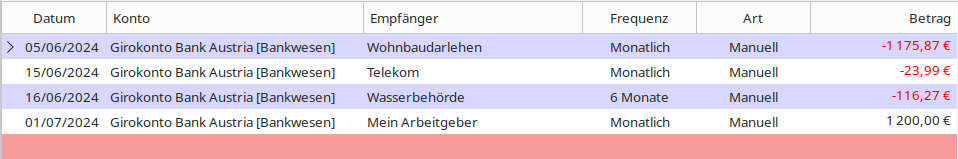
\includegraphics[width=0.95\textwidth]{image/screenshot/planned_transactions_list}
	\end{center}
	\caption{Liste der geplanten Buchungen}
	%\caption{List of scheduled transactions}
	%\caption{Liste des opérations planifiées}
	\label{planned-transactions-list-img}
\end{figure}

Oben wird die Spaltenüberschriftenleiste angezeigt. Sie können \indexword{eine Spalte verbreitern oder verengen}\index{column!width}, indem Sie auf den Trennbalken zwischen zwei Spalten klicken und ihn ziehen. Um die \indexword{Spaltenbreiten}\index{Spalte!Breiten} auf ihre Standardwerte zurückzusetzen, wählen Sie den Menüpunkt \menus{Ansicht - Spaltenbreite zurücksetzen} aus der Menüleiste.
%The column heading bar appears at the top. You can \indexword{widen or narrow a column}\index{column!width} by clicking on the separator between two columns and dragging it. To restore the \indexword{column widths}\index{column!width} to their default values, select the \menus{View – Reset the column width} menu from the menu bar.
%Elle affiche en haut la barre des libellés des colonnes. Vous pouvez \indexword{élargir ou rétrécir une colonne}\index{colonne!largeur} en cliquant sur le séparateur entre deux colonnes et en le déplaçant. Pour rétablir la \indexword{largeur des colonnes}\index{colonne!largeur} à leur valeur par défaut, sélectionnez le menu \menus{Affichage - Réinitialiser la largeur des colonnes} dans la barre de menu.

Sie können die Liste der geplanten Buchungen mit dem Mausrad oder mit der Maus und dem vertikalen Bildlaufbalken nach oben oder unten verschieben. Eine eventuelle Verschiebung nach links oder rechts erfolgt mit der Maus und dem horizontalen Bildlaufbalken.
%You can scroll the list of scheduled transactions up or down using the mouse wheel, or by using the mouse and the vertical scroll bar. To scroll left or right, use the mouse and the horizontal scroll bar.
%Vous pouvez déplacer la liste des opérations planifiées vers le haut ou vers le bas avec la molette de la souris, ou bien avec la souris et l'ascenseur vertical. Le déplacement éventuel vers la gauche ou la droite se fait avec la souris et l'ascenseur horizontal.

% espace pour changement de thème
\vspacepdf{2mm}
Jeder Buchung wird in einer einzigen Zeile und in maximal sechs Spalten angezeigt, was maximal sechs Informationsfelder für jeden geplanten Buchung ergibt. Die Anzeigefelder sowie die \indexword{Spaltenbezeichnungen}\index{Spalte!Bezeichnung} lauten wie folgt:
%Each transaction is displayed on a single line and across a maximum of six columns, providing a maximum of six information fields for each scheduled transaction. The display fields, along with the \indexword{column headings}\index{column!heading}, are as follows:
%Chaque opération est affichée sur une seule ligne et au maximum six colonnes, ce qui fait au maximum six champs d'information pour chaque opération planifiée. Les champs d'affichage, ainsi que les \indexword{libellés des colonnes}\index{colonne!libellé}, sont les suivants:
\begin{itemize}
	\item \menus{Datum}: das Datum der Buchung;
	%\item \menus{Date}: the date of the transaction;
	%\item \menus{Date}: la date de l'opération;
	\item \menus{Konto}: das betreffende Konto;
	%\item \menus{Account}: the account in question;
	%\item \menus{Compte}: le compte concerné;
	\item \menus{Empfänger}: 
	%\item \menus{Payee}: 
	%\item \menus{Tiers};
	\item \menus{Frequenz}: die Frequenz der Transaktion;
	%\item \menus{Frequency}: the frequency of the transaction;
	%\item \menus{Périodicité}: la périodicité de l'opération;
	\item \menus{Art}: die Ausführungsart, automatisch oder manuell;
	%\item \menus{Mode}: the method of execution, automatic or manual;
	%\item \menus{Mode}: le mode d'exécution, automatique ou manuel;
	\item \menus{Betrag}: den Buchungsbetrag; ein \indexword{negativer Betrag}\index{Betrag!negativ} wird in \textcolor{red}{Rot} angezeigt.
	%\item \menus{Amount}: the transaction amount; a \indexword{negative amount}\index{amount!negative} is displayed in \textcolor{red}{red}.
	%\item \menus{Montant}: le montant de l'opération; un \indexword{montant négatif}\index{montant!négatif} est affiché en \textcolor{red}{rouge}.
	% saut de ligne pour indentation correcte de la note dans la liste
	
	\Note{}: Wenn das Feld \menus{Notizen} angefordert wurde, wird es anstelle der Felder \menus{Frequenz} und \menus{Art} angezeigt, sodass nur fünf Spalten und fünf Felder angezeigt werden (siehe Abschnitt \vref{plannedtransactions-comments}, \menus{Kommentare zu geplanten Buchungen}).
	%\Note{}: if the \menus{Notes} field has been requested, it is displayed in place of the \menus{Frequency} and \menus{Method} fields, resulting in only five columns and five fields being displayed (see section \vref{plannedtransactions-comments}, \menus{Comments on planned transactions}).
	%\Note{}: si l'affichage du champ \menus{Remarques} a été demandé, il s'affiche à la place des champs \menus{Périodicité} et \menus{Mode}, ce qui ne fait plus que cinq colonnes et cinq champs affichés (voir la section \vref{plannedtransactions-comments}, \menus{Remarques des opérations planifiées}).
\end{itemize}

% espace pour changement de thème
\vspacepdf{2mm}
Direkt unterhalb der letzten Buchungszeile erscheint eine zusätzliche Leerzeile, die zum Anlegen einer neuen geplanten Buchung dient (siehe Abschnitt \vref{plannedtransactions-new}, \menus{Neue geplante Buchung}).
%An additional blank line appears just below the last transaction line and is used to create a new scheduled transaction (see section \vref{plannedtransactions-new}, \menus{New Scheduled Transaction}).
%Une ligne supplémentaire vide s'affiche juste en-dessous de la dernière ligne d'opération, et sert à créer une nouvelle opération planifiée (voir la section \vref{plannedtransactions-new}, \menus{Nouvelle opération planifiée}).

% espace pour changement de thème
\vspacepdf{2mm}
Um die Lesbarkeit der Anzeige zu verbessern, wechselt Grisbi bei jeder Zeile zwischen den Farben \colorbox[RGB]{215,215,255}{violetter Hintergrund} und Weiß.
%To improve the readability of the display, Grisbi alternates between a \colorbox[RGB]{215,215,255}{purple background} and white for each line.
%Pour des raisons de lisibilité de l'affichage, Grisbi présente une alternance de couleurs de \colorbox[RGB]{215,215,255}{fond violet} et blanc à chaque ligne.

% espace pour changement de thème
\vspacepdf{2mm}
Durch Klicken auf das Werkzeug \menus{Ansicht}\label{plannedtransactions-view} in der Symbolleiste können Sie über eine Dropdown-Liste\refimage{planned-transactions-view-select-img} zwischen verschiedenen Anzeigemodi für anstehende Buchungen \textit{ab dem heutigen Datum} wählen:
%By clicking on the \menus{View}\label{plannedtransactions-view} tool in the toolbar, a drop-down list\refimage{planned-transactions-view-select-img} allows you to choose from several display modes for upcoming transactions \textit{from today’s date}:
%En cliquant sur l'outil \menus{Affichage}\label{plannedtransactions-view} dans la barre d'outils, une liste déroulante\refimage{planned-transactions-view-select-img} vous permet de choisir plusieurs modes d'affichage des prochaines occurrences \textit{à compter de la date du jour}:
% espace avant image 5mm

\vspacepdf{5mm}
\noindent
\begin{minipage}{.65\linewidth}
	\begin{itemize}[rightmargin=.6cm]
		\item \menus{Alle Buchungen}: der nächste Termin jedes Buchung;
		%\item \menus{Unique view}: the next occurrence of each transaction;
		%\item \menus{Vue unique}: la prochaine occurrence de chaque opération;
		\item \menus{Ansicht nach Wochen}: fällig in 7 Tagen;
		%\item \menus{Week view}: due in 7 days;
		%\item \menus{Vue hebdomadaire}: à échéance de 7 jours;
		\item \menus{Ansicht nach Monaten}: innerhalb von 30 Tagen;
		%\item \menus{Month view}: within 30 days;
		%\item \menus{Vue mensuelle}: à échéance de 30 jours;
		\item \menus{Ansicht nach 2 Monaten}: innerhalb von 60 Tagen;
		%\item \menus{Two months view}: within 60 days;
		%\item \menus{Vue bimestrielle}: à échéance de 60 jours;
		\item \menus{Ansicht Vierteljährlich}: innerhalb von 90 Tagen;
		%\item \menus{Quarter view}: within 90 days;
		%\item \menus{Vue trimestrielle}: à échéance de 90 jours;
		\item \menus{Ansicht Jährlich}: innerhalb eines Jahrs;
		%\item \menus{Year view}: within one year;
		%\item \menus{Vue annuelle}: à échéance d'un an;
		\item \menus{Ansicht benutzerdefiniert}: mit einer Laufzeit von einer beliebigen Anzahl von Tagen, Wochen, Monaten oder Jahren.
		%\item \menus{Custom view}: within any number of days, weeks, months or years.
		%\item \menus{Vue personnalisée}: à échéance d'un nombre quelconque de jours, semaines, mois ou années.
		% saut de ligne pour indentation correcte de la note dans la liste
		
		\Note{}: Die aktuell angezeigte Ansicht wird durch ein Häkchen gekennzeichnet, und in Klammern wird die Anzahl der Buchungen in der ausgewählten Ansicht angezeigt.
		%\Note{}: the current view is indicated by a tick, and the number of transactions in the selected view is shown in brackets.
		%\Note{}: l'affichage courant y est indiqué par une coche et, entre parenthèses, vous avez le nombre d'opérations dans la vue sélectionnée.
	\end{itemize}
\end{minipage}
\hspace{15pt}
\begin{minipage}{.35\linewidth}
	\vspace{-5pt}
	\centering
	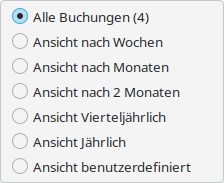
\includegraphics[width=.8\textwidth]{image/screenshot/planned_transactions_view_select}
	%\vspace{-5pt}
	\captionsetup{%						% for a change of options of the caption package
		format=plain,						% to avoid error message with labelsep option below, default=hang
		type=figure,%
		name=Fig.,%							% rename label caption, default="Figure" (or "Table")
		justification=centering,			% centring of text and caption label 
		labelsep=newline}					% define the separator between the label and the caption text
	\caption{Auswahl der Ansicht}
	%\caption{View selection}
	%\caption{Choix d'affichage}
	\vspace{-10pt}
	\label{planned-transactions-view-select-img}
\end{minipage}	

\vspacepdf{5mm}
Wenn Sie \menus{Ansicht benutzerdefiniert} wählen, öffnet sich ein neues Fenster mit einem Eingabefeld zur Auswahl der Anzahl der Zeiträume und einer Dropdown-Liste für die Art des gewünschten Zeitraums.
%If you select \menus{Custom view}, a new window will appear showing an incremental field to select the number of periods and a drop-down list for the type of period required\refimage{planned-transactions-view-custom-img}.
%Si vous choisissez \menus{Vue personnalisée}, une nouvelle fenêtre affiche un champ incrémental pour choisir le nombre de périodes et une liste déroulante pour le type de la période désirée\refimage{planned-transactions-view-custom-img}.

% image centrée 
\begin{figure}[htbp]
	\begin{center}
		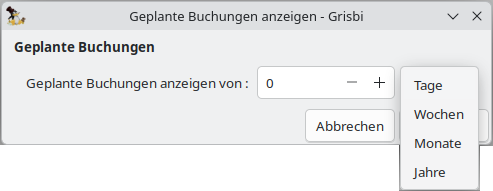
\includegraphics[width=0.5\textwidth]{image/screenshot/planned_transactions_view_custom}
	\end{center}
	\vspace{-10pt}
	\caption{Auswahl der Darstellung des benutzerdefinierten Zeitraums}
	%\caption{Selecting the custom period view}
	%\caption{Choix de l'affichage de la période personnalisée}
	\vspace{-10pt}
	\label{planned-transactions-view-custom-img}
\end{figure}
% image centrée 


%TODO following
